\begin{enumerate}[label=\thesection.\arabic*.,ref=\thesection.\theenumi]
\numberwithin{equation}{enumi}


\item Fig. \ref{fig:ee18btech11019_hart} shows a
Hartley oscillator built using opamp.  Draw the equivalent block diagram.
\begin{figure}[ht]
    \begin{center}
	    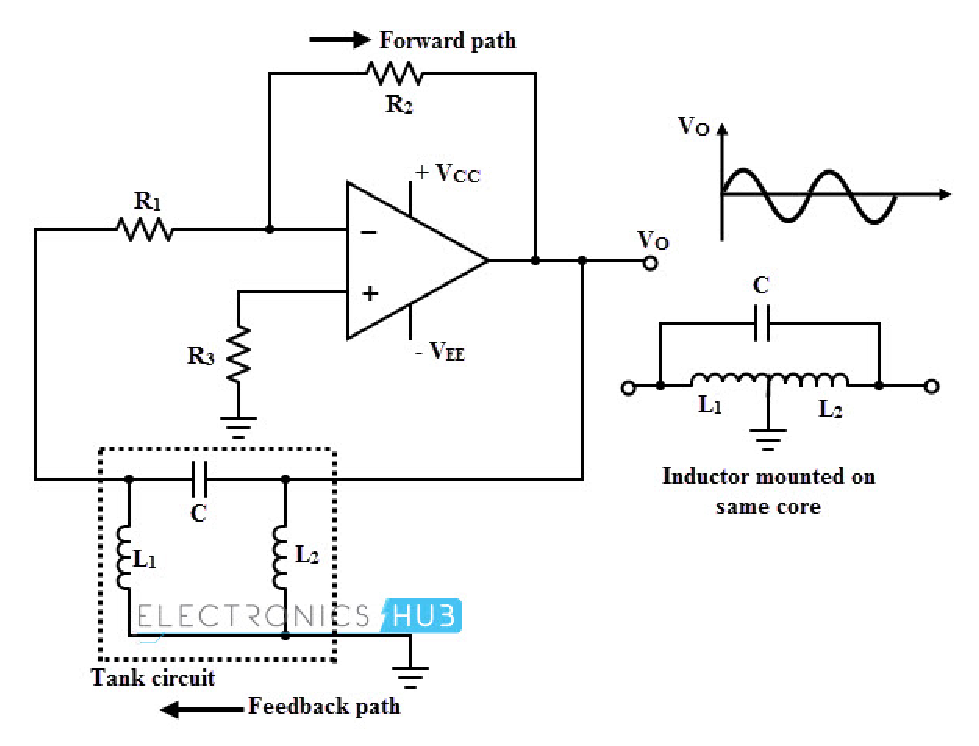
\includegraphics[width=\columnwidth]{./figs/ee18btech11019/hart.eps}
	\end{center}
\caption{block diagram for oscillator}
\label{fig:ee18btech11019_hart}
\end{figure}
\\
\solution Fig. \label{fig:ee18btech11019_hart_block} shows the block diagram of the Hartley Oscillator in Fig. \ref{fig:ee18btech11019_hart}.
\begin{figure}[!ht]
    \begin{center}
		
		\resizebox{\columnwidth}{!}{\tikzset{
        amp/.style = {regular polygon, regular polygon sides=3,
              draw, fill=white, text width=1em,
              inner sep=1mm, outer sep=0mm,
              shape border rotate=-90},
        block/.style = {draw, rectangle,
            minimum height=1cm,
            minimum width=2cm},
        input/.style = {coordinate,node distance=1cm},
        output/.style = {coordinate,node distance=4cm},
        arrow/.style={draw, -latex,node distance=2cm},
        pinstyle/.style = {pin edge={latex-, black,node distance=2cm}},
        sum/.style = {draw, circle, node distance=1cm},
}

\begin{tikzpicture}[node distance=2.5cm,auto,>=latex']
  \node [input, name=input] {};
  \node [sum, right of=input] (sum) {};
  \node [amp, right of = sum] (block1) {$G$};
  \node [output, right of= block1] (output) {};
  \node [block, below of = block1] (block2) {$H$};
  \draw [->] (input) -- node {$V_{in}$} (sum);
  \draw [->] (sum) -- node {$V_{in} + HV_{out}$} (block1);
  \draw [->] (block1) -- node [name =y] {$V_{out}$} (output);
  \draw [->] (y) |- node [above,pos=0.79] {$V_{out}$} (block2) ;
  \draw [->] (block2) -| node  {$HV_{out}$} (sum) ;
\end{tikzpicture}
}
	\end{center}
\caption{block diagram for oscillator}
\label{fig:ee18btech11019_hart_block}
\end{figure}

\item Show that the gain of the oscillator is 
\begin{align}
    G = \frac{V_{out}}{V_{in}} = \frac{A}{1 - AB}
\label{eq:ee18btech11019_gain}
\end{align}
%
\\
\solution From \ref{fig:ee18btech11019_hart_block}
%
\begin{align}
    A(V_{in} + BV_{out}) =V_{out} 
\end{align}
%
resulting in \eqref{eq:ee18btech11019_gain}.
\item State the condition for sustained oscillations. Justify.
\item Find $A$ and $B$.
\item Find the frequency of oscillation using the condition that $AB = 1$.
%


%a Hartley Oscillator.
%shows the  block diagram of a Hartley Oscillator.
%\begin{figure}[!ht]
%    \begin{center}
%		
%		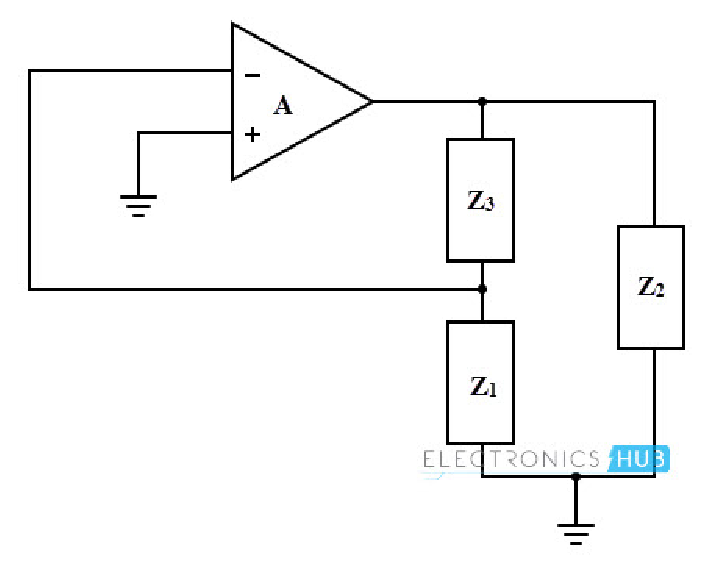
\includegraphics[width=\columnwidth]{./figs/ee18btech11019/blc.eps}
%	\end{center}
%\caption{block diagram for oscillator}
%\label{fig:ee18btech11019_block2}
%\end{figure}

%\solution Oscillators convert a DC input (the supply voltage) into an AC output (the waveform) \\
Given Below is basic block diagram\\
Resonant frequency, is the frequency at which oscillator oscillates, it depends on R/L/C components of the circuit it's been fed back through.\\
Oscillators work because they overcome the losses of their positive feedback circuit either in the form of a capacitor, inductor or both. In other words, an oscillator is a an amplifier which uses positive feedback that generates an output frequency without the use of an input signal.\\
Oscillators gain can be given as follows:\\
\item Hartley oscillator:\\
The Hartley oscillator is one of the classical LC feedback circuits,i.e feedback is made of LC components.Below here we can see a general form of any LC-type oscillator:


For any LC oscillator, 
\begin{align}
    Z_1 = jX_1\\
    Z_2 = jX_2\\
    Z_3 = jX_3\\
\end{align}
We know that feedback gain is B, i.e, $\frac{V_0}{V_f} = B$\\
Applyting voltage divider rule we get
\begin{align}
    B = \frac{Z_1}{Z_1 + Z_3}
\end{align}
Consider the below circuit
\begin{figure}[!ht]
    \begin{center}
		
		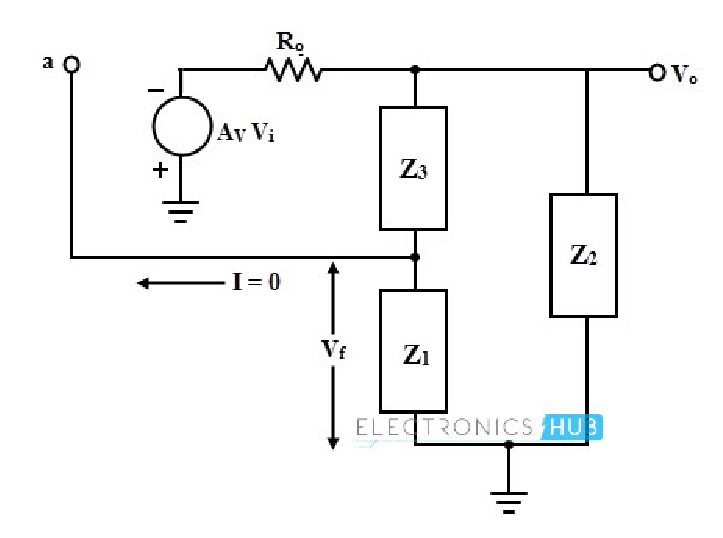
\includegraphics[width=\columnwidth]{./figs/ee18btech11019/lc.eps}
	\end{center}
\caption{block diagram for oscillator}
\label{fig:ee18btech11019_block2}
\end{figure}
\begin{align}
    A = \frac{V_o}{V_{in}} = \frac{AZ_L}{R_o + Z_L}\\
    where\\
    Z_L = \frac{(Z_2 + Z_3)Z_1}{Z_1+Z_2+Z_3}\\
\end{align}
Now,we know that $AB = 1$ for sustained oscillations, putting the the above terms in the equation

    on solving,\\
\begin{align}    
    AB = \frac{Z_1Z_2A}{(Z_1+Z_2+Z_3)A+ Z_1(Z_2+Z_3)}\\
    Z_1 = jX_1,
    Z_2 = jX_2,
    Z_3 = jX_3\\
\end{align}    

    putting that in we get\\
\begin{align}
AB = \frac{AX_1X_2}{X_1(X_2+X_3) -jR_o(X_1+X_2+X_3)}
\end{align}
For hartley oscillator, 
\begin{align}
    Z_1 = j\omega L_1 (inductor)\\
    Z_2 = j\omega L_2 (inductor)\\
    Z_3 = \frac{1}{j\omega C} (capacitor)\\
\end{align}
Since, AB is real
\begin{align}
    X_1+X_2+X_3 = 0\\
\end{align}

    For, Hartley oscillator, substituting terms in above equation\\
\begin{align}    
    \omega L_1 + \omega L_2  = \frac{1}{\omega C}\\
    \omega = \frac{1}{\sqrt{(L_1+L_2)(C)}}\\
    f = \frac{1}{2\pi \sqrt{(L_1+L_2)(C)}}
\end{align}
\begin{align}
    B = \frac{Z_1}{Z_1 + Z_3} = \frac{Z_1}{Z_2}\\
      = \frac{L_1}{L_2}\\
    A =  \frac{L_2}{L_1} 
\end{align}
Given below is circuit for 
\item For Hartley oscillator frequency generated can be given as 
\begin{align}
    f = \frac{1}{2\pi\sqrt{(L_1 + L_2)C}}
\end{align}
Taking,
\begin{align}
   L_1 = 1 \mu H\\
   L_2 = 1 \mu H\\
   C = 1.2 pF
\end{align}
We get f = 103 MHz\\
Feedback factor for Hartley given by:
\begin{align}
Feedback factor =\frac{L_2}{L_1}= 1
\end{align}
W.K.T, $AB = 1$\\
$\therefore$ Minimum amplification Gain = 1
\end{enumerate}
